\documentclass{article}
\usepackage {inputenc, fullpage, listings, amsmath, graphicx}

\parindent 0pt

\title{%
   CSc 226: Operating Systems (Spring 2022) \\
   \large Written Assignment 3\\
    Alex Holland V00}
    
\date{}

\begin{document}

\maketitle

{\bf Question 1}\\
Constructed Graph:

\begin{center}
    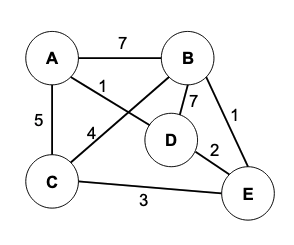
\includegraphics[width=.4\textwidth]{1.png}
\end{center}

{\bf (a)}\\
$(node \; v, \; D(v))$\\
Distance after initialization: $(A, 0), (B,+\infty), (C,+\infty), (D,+\infty), (E,+\infty)$\\


Vertex A is added, distance values are: $(A, 0), (B,7), (C,5), (D,1), (E,+\infty)$

\begin{center}
    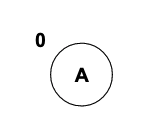
\includegraphics[width=.2\textwidth]{1a-1.png}
\end{center}

Vertex D is added, distance values are: $(A, 0), (B,7), (C,5), (D,1), (E,2)$

\begin{center}
    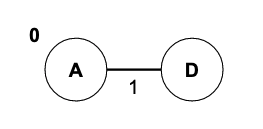
\includegraphics[width=.3\textwidth]{1a-2.png}
\end{center}

Vertex E is added, distance values are: $(A, 0), (B,1), (C,3), (D,1), (E,2)$

\begin{center}
    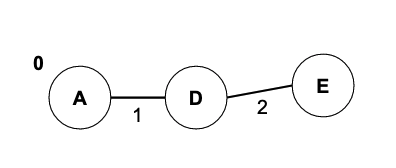
\includegraphics[width=.4\textwidth]{1a-3.png}
\end{center}

Vertex B is added, distance values are: $(A, 0), (B,1), (C,3), (D,1), (E,2)$

\begin{center}
    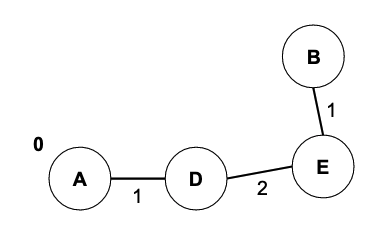
\includegraphics[width=.4\textwidth]{1a-4.png}
\end{center}

Vertex C is added, distance values are: $(A, 0), (B,1), (C,3), (D,1), (E,2)$

\begin{center}
    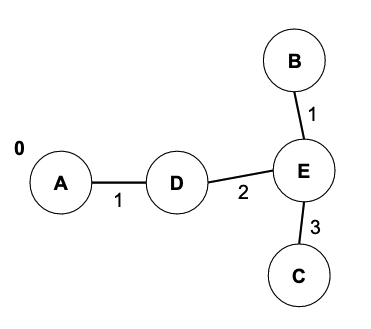
\includegraphics[width=.4\textwidth]{1a-5.png}
\end{center}

{\bf (b)}\\
{\bf i)}\\
The edges and nodes are added to the tree in the following order:
\begin{enumerate}
    \item Vertex A and D are connected via the edge (A, D, 1).
    \item Vertex B and E are connected via the edge (B, E, 1).
    \item The two trees are connected.
    \item Vertex D is connected via the edge (D, E, 2).
    \item Vertex C is connected via the edge (C, E, 3).
\end{enumerate}

\bigskip

{\bf ii)}\\
Initialization:
\begin{center}
    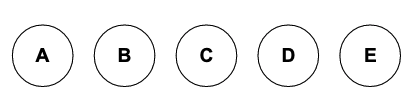
\includegraphics[width=.45\textwidth]{1b-1.png}
\end{center}

Edge (A,D,1) is added:
\begin{center}
    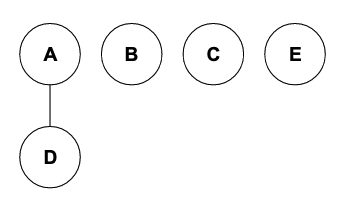
\includegraphics[width=.35\textwidth]{1b-2.png}
\end{center}

Edge (B,E,1) is added:
\begin{center}
    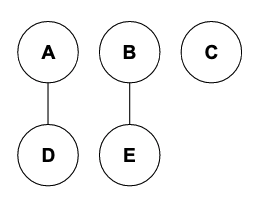
\includegraphics[width=.3\textwidth]{1b-3.png}
\end{center}

Edge (D,E,2) is added:
\begin{center}
    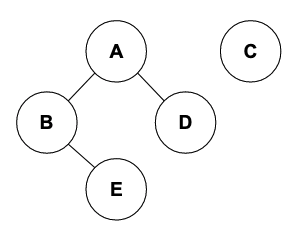
\includegraphics[width=.35\textwidth]{1b-4.png}
\end{center}

Edge (C,E,C) is added:
\begin{center}
    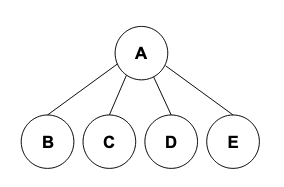
\includegraphics[width=.35\textwidth]{1b-5.png}
\end{center}

{\bf Question 2}\\
{\bf a)}\\
To show that we can rescale the edge weights of a graph G by adding a positive constant to all of them without affecting the MST lets consider the graph from Question 1:

\smallskip
$(A,B,7),(A,C,5),(A,D,1),(B,C,4),(B,D,7),(B,E,1),(C,E,3),(D,E,2)$

\begin{center}
    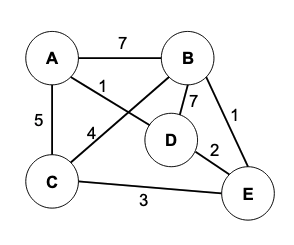
\includegraphics[width=.4\textwidth]{1.png}
\end{center}

As determined in Question 1a, the minimum spanning tree using Prim's algorithm is:

\begin{center}
    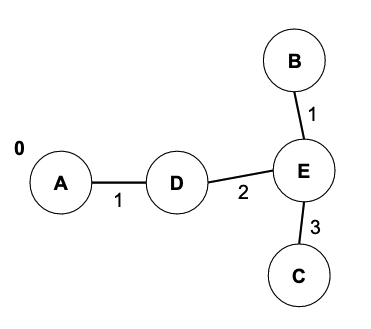
\includegraphics[width=.4\textwidth]{1a-5.png}
\end{center}

Lets add a positive constant $(N)$, say $N=3$. So the new weighted edges are:\\ $(A,B,10),(A,C,8),(A,D,4),(B,C,7),(B,D,10),(B,E,4),(C,E,6),(D,E,5)$\\

\begin{center}
    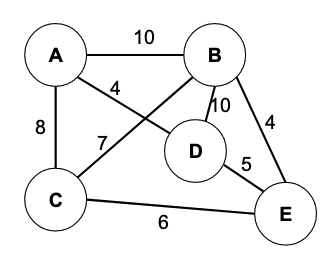
\includegraphics[width=.4\textwidth]{2a-1.png}
\end{center}

Now lets determine the minimum spanning tree using Prim's algorithm:

\smallskip
First node is A.

\begin{center}
    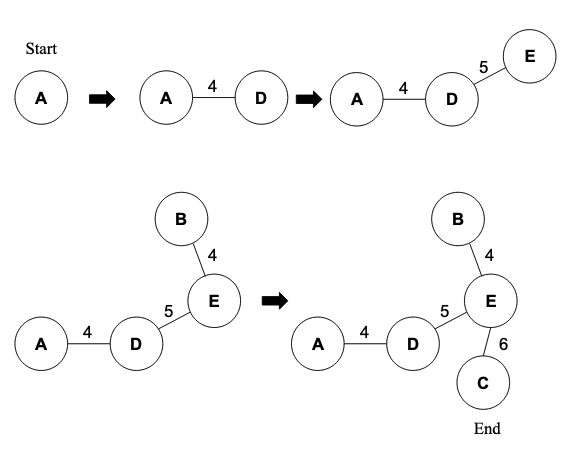
\includegraphics[width=1\textwidth]{2a-2.png}
\end{center}

As shown by adding a positive constant to all of the edge weights the MST between the original and rescaled graph is not affected. This would work for any positive constant since the weighting of each edge would be increased by the same amount, so no edge would change such that one has a higher or lower priority over another when recalculating the MST.

\bigskip
{\bf b)}\\
Prim's and Kruskal's algorithm still work correctly if the graph $G$ contains edges with negative weights. In Prim's algorithm the safe edge added is always the least-weighted edge connecting the tree to a vertex not in the tree. Likewise, Kruskals' algorithm takes the least weighted edge in the graph that connects two distinct components. Therefore, both algorithms work correctly with negative edge weights since the Prim's and Kruskal's algorithm takes the lightweight edge, whether it be negative or positive. Let's observe the graph in graph from question 1 with each edge weight set to be negative:\\


Nodes $V={A,B,C,D,E}$ and weighted edges\\
$(A,B,-7),(A,C,-5),(A,D,-1),(B,C,4-),(B,D,-7),(B,E,-1),(C,E,-3),(D,E,-2)$\\

\smallskip
First Node is A
\begin{center}
    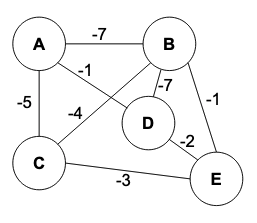
\includegraphics[width=.4\textwidth]{4.png}
\end{center}

Prim's algorithm:
\begin{center}
    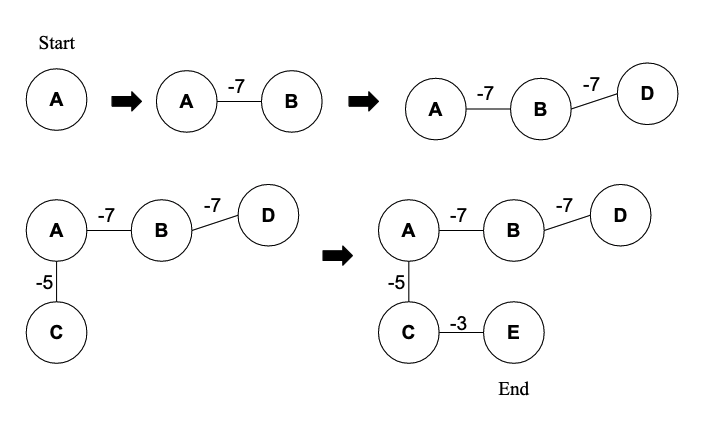
\includegraphics[width=1\textwidth]{4-1.png}
\end{center}

Kruskal's algorithm (no path compression):
\begin{center}
    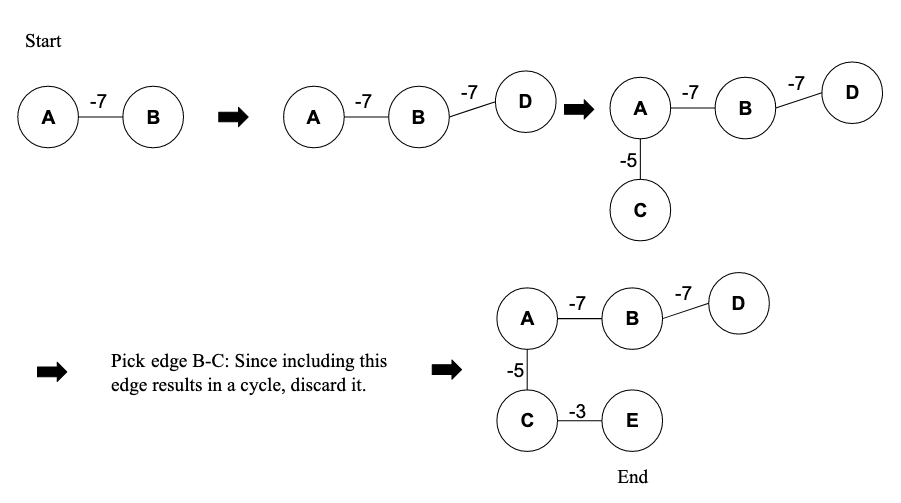
\includegraphics[width=1\textwidth]{4-2.png}
\end{center}

As shown, if a graph contains edges with negative weights, Prim's and Kruskals algorithm still works correctly and can create a MST.

\bigskip
{\bf Question 3}\\
Suppose that all edge weights in a graph are integers in the range from 1 to $|V|$ where $V$ is the set of vertices. Let $M$ represent the number of edges. Kruskal's Algorithm takes $O(V)$ time for initialization of each single set. Since we know that all of the edge weights in the graph are in the the range of 1 to $|V|$, sorting will take $O(V + M)$ using a bucket sort implementation. The disjoint-set operations to determine safe edges is still $O(Mlog(V))$. Kruskals algorithm will run in $O(V+(V+M)+Mlog(V))=O(2V+M+Mlog(V))$ time, which in terms of big O time can be represented as $O(Mlog(V)$ time.

\bigskip
{\bf Question 4}\\
We want an algorithm that will find the MST for a connected graph which has had an edge deleted from it without having to construct a new tree:
\begin{lstlisting}
If the edge is not in the MST:
    new MST = old MST
If the deleted edge from the MST leaves two connected components (Sub1 & Sub2):
    Iterate until an edge with minimum weight linking Sub1 is found
        add the minimum weight edge with a vertex in Sub1
    Iterate until an edge with minimum weight linking Sub2 is found
        add the minimum weight edge with one vertex in Sub2
    
\end{lstlisting}
The algorithm require the edges to be searched by iterating through the two components in order to find the edge with minimum weight linking Sub1 and Sub2, thus the running time of this algorithm would be O(m).

\end{document}
